\documentclass{article}
\usepackage{xcolor}
\usepackage{tcolorbox}


\begin{document}

\begin{tcolorbox}[colback=red!10,colframe=red!80,width=\textwidth,arc=3mm,auto outer arc]
\centering
{\Huge \textbf{\textsc{Error}}}\
\Large The LaTeX code was generated successfully, but the compilation was unsuccessful.
\end{tcolorbox}


\noindent You can copy the source of the LaTeX or try to regenerate and recompile.
\vspace{2.5em}
\begin{tcolorbox}[colback=white,colframe=black,boxrule=1pt,width=\textwidth,arc=3mm,auto outer arc]
    \begin{center}
        \textbf{FUN FACT}
    \end{center}
\begin{center}
	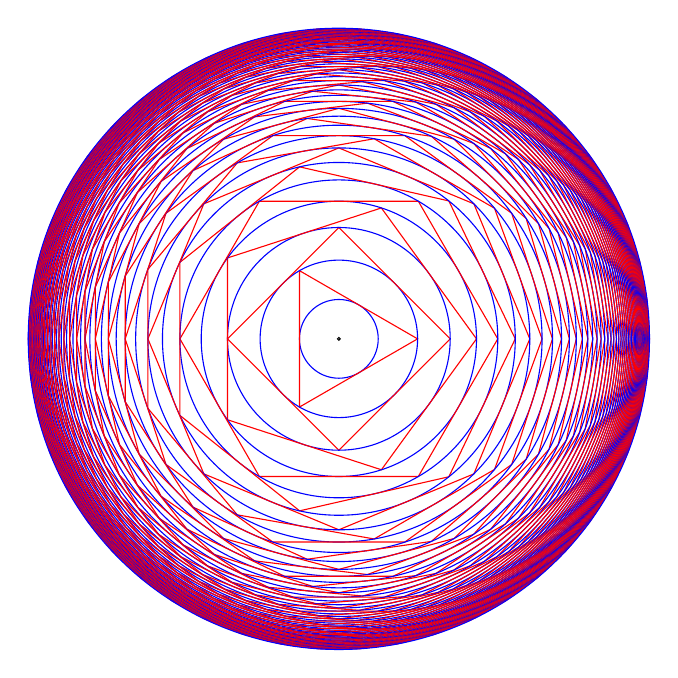
\begin{tikzpicture}[scale=0.5]
\draw (0,0) circle (1pt);
\draw[blue] (0,0) circle (1);
\draw[red] (2.000000,0.000000) -- (-1.000000,1.732051) -- (-1.000000,-1.732051) -- cycle;
\draw[blue] (0,0) circle (2.000000);
\draw[red] (2.828427,0.000000) -- (0.000000,2.828427) -- (-2.828427,0.000000) -- (-0.000000,-2.828427) -- cycle;
\draw[blue] (0,0) circle (2.828427);
\draw[red] (3.496128,0.000000) -- (1.080363,3.325016) -- (-2.828427,2.054973) -- (-2.828427,-2.054973) -- (1.080363,-3.325016) -- cycle;
\draw[blue] (0,0) circle (3.496128);
\draw[red] (4.036981,0.000000) -- (2.018491,3.496128) -- (-2.018491,3.496128) -- (-4.036981,0.000000) -- (-2.018491,-3.496128) -- (2.018491,-3.496128) -- cycle;
\draw[blue] (0,0) circle (4.036981);
\draw[red] (4.480711,0.000000) -- (2.793678,3.503161) -- (-0.997052,4.368370) -- (-4.036981,1.944108) -- (-4.036981,-1.944108) -- (-0.997052,-4.368370) -- (2.793678,-3.503161) -- cycle;
\draw[blue] (0,0) circle (4.480711);
\draw[red] (4.849887,0.000000) -- (3.429388,3.429388) -- (0.000000,4.849887) -- (-3.429388,3.429388) -- (-4.849887,0.000000) -- (-3.429388,-3.429388) -- (-0.000000,-4.849887) -- (3.429388,-3.429388) -- cycle;
\draw[blue] (0,0) circle (4.849887);
\draw[red] (5.161142,0.000000) -- (3.953664,3.317518) -- (0.896223,5.082732) -- (-2.580571,4.469680) -- (-4.849887,1.765214) -- (-4.849887,-1.765214) -- (-2.580571,-4.469680) -- (0.896223,-5.082732) -- (3.953664,-3.317518) -- cycle;
\draw[blue] (0,0) circle (5.161142);
\draw[red] (5.426745,0.000000) -- (4.390329,3.189761) -- (1.676957,5.161142) -- (-1.676957,5.161142) -- (-4.390329,3.189761) -- (-5.426745,0.000000) -- (-4.390329,-3.189761) -- (-1.676957,-5.161142) -- (1.676957,-5.161142) -- (4.390329,-3.189761) -- cycle;
\draw[blue] (0,0) circle (5.426745);
\draw[red] (5.655847,0.000000) -- (4.758001,3.057782) -- (2.349524,5.144739) -- (-0.804911,5.598279) -- (-3.703792,4.274404) -- (-5.426745,1.593436) -- (-5.426745,-1.593436) -- (-3.703792,-4.274404) -- (-0.804911,-5.598279) -- (2.349524,-5.144739) -- (4.758001,-3.057782) -- cycle;
\draw[blue] (0,0) circle (5.655847);
\draw[red] (5.855364,0.000000) -- (5.070894,2.927682) -- (2.927682,5.070894) -- (0.000000,5.855364) -- (-2.927682,5.070894) -- (-5.070894,2.927682) -- (-5.855364,0.000000) -- (-5.070894,-2.927682) -- (-2.927682,-5.070894) -- (-0.000000,-5.855364) -- (2.927682,-5.070894) -- (5.070894,-2.927682) -- cycle;
\draw[blue] (0,0) circle (5.855364);
\draw[red] (6.030602,0.000000) -- (5.339833,2.802560) -- (3.425772,4.963088) -- (0.726909,5.986632) -- (-2.138481,5.638711) -- (-4.513970,3.999029) -- (-5.855364,1.443218) -- (-5.855364,-1.443218) -- (-4.513970,-3.999029) -- (-2.138481,-5.638711) -- (0.726909,-5.986632) -- (3.425772,-4.963088) -- (5.339833,-2.802560) -- cycle;
\draw[blue] (0,0) circle (6.030602);
\draw[red] (6.185690,0.000000) -- (5.573114,2.683870) -- (3.856715,4.836167) -- (1.376446,6.030602) -- (-1.376446,6.030602) -- (-3.856715,4.836167) -- (-5.573114,2.683870) -- (-6.185690,0.000000) -- (-5.573114,-2.683870) -- (-3.856715,-4.836167) -- (-1.376446,-6.030602) -- (1.376446,-6.030602) -- (3.856715,-4.836167) -- (5.573114,-2.683870) -- cycle;
\draw[blue] (0,0) circle (6.185690);
\draw[red] (6.323882,0.000000) -- (5.777154,2.572155) -- (4.231503,4.699560) -- (1.954187,6.014369) -- (-0.661026,6.289239) -- (-3.161941,5.476643) -- (-5.116128,3.717085) -- (-6.185690,1.314809) -- (-6.185690,-1.314809) -- (-5.116128,-3.717085) -- (-3.161941,-5.476643) -- (-0.661026,-6.289239) -- (1.954187,-6.014369) -- (4.231503,-4.699560) -- (5.777154,-2.572155) -- cycle;
\draw[blue] (0,0) circle (6.323882);
\draw[red] (6.447774,0.000000) -- (5.956967,2.467456) -- (4.559265,4.559265) -- (2.467456,5.956967) -- (0.000000,6.447774) -- (-2.467456,5.956967) -- (-4.559265,4.559265) -- (-5.956967,2.467456) -- (-6.447774,0.000000) -- (-5.956967,-2.467456) -- (-4.559265,-4.559265) -- (-2.467456,-5.956967) -- (-0.000000,-6.447774) -- (2.467456,-5.956967) -- (4.559265,-4.559265) -- (5.956967,-2.467456) -- cycle;
\draw[blue] (0,0) circle (6.447774);
\draw[red] (6.559462,0.000000) -- (6.116516,2.369551) -- (4.847501,4.419081) -- (2.923804,5.871789) -- (0.605231,6.531480) -- (-1.795082,6.309058) -- (-3.952959,5.234563) -- (-5.576967,3.453112) -- (-6.447774,1.205298) -- (-6.447774,-1.205298) -- (-5.576967,-3.453112) -- (-3.952959,-5.234563) -- (-1.795082,-6.309058) -- (0.605231,-6.531480) -- (2.923804,-5.871789) -- (4.847501,-4.419081) -- (6.116516,-2.369551) -- cycle;
\draw[blue] (0,0) circle (6.559462);
\draw[red] (6.660652,0.000000) -- (6.258965,2.278077) -- (5.102355,4.281384) -- (3.330326,5.768294) -- (1.156610,6.559462) -- (-1.156610,6.559462) -- (-3.330326,5.768294) -- (-5.102355,4.281384) -- (-6.258965,2.278077) -- (-6.660652,0.000000) -- (-6.258965,-2.278077) -- (-5.102355,-4.281384) -- (-3.330326,-5.768294) -- (-1.156610,-6.559462) -- (1.156610,-6.559462) -- (3.330326,-5.768294) -- (5.102355,-4.281384) -- (6.258965,-2.278077) -- cycle;
\draw[blue] (0,0) circle (6.660652);
\draw[red] (6.752751,0.000000) -- (6.386868,2.192615) -- (5.328869,4.147625) -- (3.693404,5.653176) -- (1.657702,6.546118) -- (-0.557638,6.729686) -- (-2.712549,6.183989) -- (-4.573513,4.968160) -- (-5.938867,3.213954) -- (-6.660652,1.111466) -- (-6.660652,-1.111466) -- (-5.938867,-3.213954) -- (-4.573513,-4.968160) -- (-2.712549,-6.183989) -- (-0.557638,-6.729686) -- (1.657702,-6.546118) -- (3.693404,-5.653176) -- (5.328869,-4.147625) -- (6.386868,-2.192615) -- cycle;
\draw[blue] (0,0) circle (6.752751);
\draw[red] (6.836924,0.000000) -- (6.502302,2.112726) -- (5.531188,4.018643) -- (4.018643,5.531188) -- (2.112726,6.502302) -- (0.000000,6.836924) -- (-2.112726,6.502302) -- (-4.018643,5.531188) -- (-5.531188,4.018643) -- (-6.502302,2.112726) -- (-6.836924,0.000000) -- (-6.502302,-2.112726) -- (-5.531188,-4.018643) -- (-4.018643,-5.531188) -- (-2.112726,-6.502302) -- (-0.000000,-6.836924) -- (2.112726,-6.502302) -- (4.018643,-5.531188) -- (5.531188,-4.018643) -- (6.502302,-2.112726) -- cycle;
\draw[blue] (0,0) circle (6.836924);
\draw[red] (6.914150,0.000000) -- (6.606973,2.037981) -- (5.712739,3.894879) -- (4.310902,5.405700) -- (2.526023,6.436201) -- (0.516695,6.894816) -- (-1.538543,6.740798) -- (-3.457075,5.987829) -- (-5.068430,4.702816) -- (-6.229434,2.999937) -- (-6.836924,1.030501) -- (-6.836924,-1.030501) -- (-6.229434,-2.999937) -- (-5.068430,-4.702816) -- (-3.457075,-5.987829) -- (-1.538543,-6.740798) -- (0.516695,-6.894816) -- (2.526023,-6.436201) -- (4.310902,-5.405700) -- (5.712739,-3.894879) -- (6.606973,-2.037981) -- cycle;
\draw[blue] (0,0) circle (6.914150);
\draw[red] (6.985250,0.000000) -- (6.702298,1.967972) -- (5.876366,3.776511) -- (4.574366,5.279099) -- (2.901778,6.354006) -- (0.994105,6.914150) -- (-0.994105,6.914150) -- (-2.901778,6.354006) -- (-4.574366,5.279099) -- (-5.876366,3.776511) -- (-6.702298,1.967972) -- (-6.985250,0.000000) -- (-6.702298,-1.967972) -- (-5.876366,-3.776511) -- (-4.574366,-5.279099) -- (-2.901778,-6.354006) -- (-0.994105,-6.914150) -- (0.994105,-6.914150) -- (2.901778,-6.354006) -- (4.574366,-5.279099) -- (5.876366,-3.776511) -- (6.702298,-1.967972) -- cycle;
\draw[blue] (0,0) circle (6.985250);
\draw[red] (7.050922,0.000000) -- (6.789455,1.902316) -- (6.024445,3.663546) -- (4.812629,5.153068) -- (3.243883,6.260410) -- (1.434553,6.903446) -- (-0.481172,7.034485) -- (-2.361210,6.643808) -- (-4.066128,5.760391) -- (-5.469480,4.449752) -- (-6.467186,2.809095) -- (-6.985250,0.960100) -- (-6.985250,-0.960100) -- (-6.467186,-2.809095) -- (-5.469480,-4.449752) -- (-4.066128,-5.760391) -- (-2.361210,-6.643808) -- (-0.481172,-7.034485) -- (1.434553,-6.903446) -- (3.243883,-6.260410) -- (4.812629,-5.153068) -- (6.024445,-3.663546) -- (6.789455,-1.902316) -- cycle;
\draw[blue] (0,0) circle (7.050922);
\draw[red] (7.111764,0.000000) -- (6.869437,1.840660) -- (6.158969,3.555882) -- (5.028777,5.028777) -- (3.555882,6.158969) -- (1.840660,6.869437) -- (0.000000,7.111764) -- (-1.840660,6.869437) -- (-3.555882,6.158969) -- (-5.028777,5.028777) -- (-6.158969,3.555882) -- (-6.869437,1.840660) -- (-7.111764,0.000000) -- (-6.869437,-1.840660) -- (-6.158969,-3.555882) -- (-5.028777,-5.028777) -- (-3.555882,-6.158969) -- (-1.840660,-6.869437) -- (-0.000000,-7.111764) -- (1.840660,-6.869437) -- (3.555882,-6.158969) -- (5.028777,-5.028777) -- (6.158969,-3.555882) -- (6.869437,-1.840660) -- cycle;
\draw[blue] (0,0) circle (7.111764);
\draw[red] (7.168288,0.000000) -- (6.943083,1.782681) -- (6.281619,3.453349) -- (5.225457,4.907031) -- (3.840961,6.052386) -- (2.215123,6.817447) -- (0.450101,7.154143) -- (-1.343203,7.041318) -- (-3.052109,6.486061) -- (-4.569239,5.523261) -- (-5.799267,4.213414) -- (-6.664906,2.638823) -- (-7.111764,0.898425) -- (-7.111764,-0.898425) -- (-6.664906,-2.638823) -- (-5.799267,-4.213414) -- (-4.569239,-5.523261) -- (-3.052109,-6.486061) -- (-1.343203,-7.041318) -- (0.450101,-7.154143) -- (2.215123,-6.817447) -- (3.840961,-6.052386) -- (5.225457,-4.907031) -- (6.281619,-3.453349) -- (6.943083,-1.782681) -- cycle;
\draw[blue] (0,0) circle (7.168288);
\draw[red] (7.220937,0.000000) -- (7.011110,1.728083) -- (6.393822,3.355737) -- (5.404949,4.788367) -- (4.101960,5.942715) -- (2.560580,6.751694) -- (0.870388,7.168288) -- (-0.870388,7.168288) -- (-2.560580,6.751694) -- (-4.101960,5.942715) -- (-5.404949,4.788367) -- (-6.393822,3.355737) -- (-7.011110,1.728083) -- (-7.220937,0.000000) -- (-7.011110,-1.728083) -- (-6.393822,-3.355737) -- (-5.404949,-4.788367) -- (-4.101960,-5.942715) -- (-2.560580,-6.751694) -- (-0.870388,-7.168288) -- (0.870388,-7.168288) -- (2.560580,-6.751694) -- (4.101960,-5.942715) -- (5.404949,-4.788367) -- (6.393822,-3.355737) -- (7.011110,-1.728083) -- cycle;
\draw[blue] (0,0) circle (7.220937);
\draw[red] (7.270095,0.000000) -- (7.074129,1.676599) -- (6.496794,3.262813) -- (5.569216,4.673127) -- (4.341400,5.831512) -- (2.879538,6.675518) -- (1.262439,7.159646) -- (-0.422718,7.257795) -- (-2.085087,6.964675) -- (-3.635047,6.296087) -- (-4.989042,5.288075) -- (-6.074076,3.994982) -- (-6.831655,2.486519) -- (-7.220937,0.844007) -- (-7.220937,-0.844007) -- (-6.831655,-2.486519) -- (-6.074076,-3.994982) -- (-4.989042,-5.288075) -- (-3.635047,-6.296087) -- (-2.085087,-6.964675) -- (-0.422718,-7.257795) -- (1.262439,-7.159646) -- (2.879538,-6.675518) -- (4.341400,-5.831512) -- (5.569216,-4.673127) -- (6.496794,-3.262813) -- (7.074129,-1.676599) -- cycle;
\draw[blue] (0,0) circle (7.270095);
\draw[red] (7.316097,0.000000) -- (7.132667,1.627985) -- (6.591576,3.174336) -- (5.719955,4.561512) -- (4.561512,5.719955) -- (3.174336,6.591576) -- (1.627985,7.132667) -- (0.000000,7.316097) -- (-1.627985,7.132667) -- (-3.174336,6.591576) -- (-4.561512,5.719955) -- (-5.719955,4.561512) -- (-6.591576,3.174336) -- (-7.132667,1.627985) -- (-7.316097,0.000000) -- (-7.132667,-1.627985) -- (-6.591576,-3.174336) -- (-5.719955,-4.561512) -- (-4.561512,-5.719955) -- (-3.174336,-6.591576) -- (-1.627985,-7.132667) -- (-0.000000,-7.316097) -- (1.627985,-7.132667) -- (3.174336,-6.591576) -- (4.561512,-5.719955) -- (5.719955,-4.561512) -- (6.591576,-3.174336) -- (7.132667,-1.627985) -- cycle;
\draw[blue] (0,0) circle (7.316097);
\draw[red] (7.359237,0.000000) -- (7.187182,1.582018) -- (6.679063,3.090064) -- (5.858638,4.453621) -- (4.764269,5.608931) -- (3.447129,6.501975) -- (1.968805,7.090993) -- (0.398421,7.348444) -- (-1.190592,7.262290) -- (-2.723934,6.836560) -- (-4.129909,6.091160) -- (-5.342773,5.060943) -- (-6.305815,3.794083) -- (-6.974004,2.349816) -- (-7.316097,0.795674) -- (-7.316097,-0.795674) -- (-6.974004,-2.349816) -- (-6.305815,-3.794083) -- (-5.342773,-5.060943) -- (-4.129909,-6.091160) -- (-2.723934,-6.836560) -- (-1.190592,-7.262290) -- (0.398421,-7.348444) -- (1.968805,-7.090993) -- (3.447129,-6.501975) -- (4.764269,-5.608931) -- (5.858638,-4.453621) -- (6.679063,-3.090064) -- (7.187182,-1.582018) -- cycle;
\draw[blue] (0,0) circle (7.359237);
\draw[red] (7.399774,0.000000) -- (7.238071,1.538500) -- (6.760030,3.009759) -- (5.986543,4.349478) -- (4.951415,5.499104) -- (3.699887,6.408392) -- (2.286656,7.037603) -- (0.773487,7.359237) -- (-0.773487,7.359237) -- (-2.286656,7.037603) -- (-3.699887,6.408392) -- (-4.951415,5.499104) -- (-5.986543,4.349478) -- (-6.760030,3.009759) -- (-7.238071,1.538500) -- (-7.399774,0.000000) -- (-7.238071,-1.538500) -- (-6.760030,-3.009759) -- (-5.986543,-4.349478) -- (-4.951415,-5.499104) -- (-3.699887,-6.408392) -- (-2.286656,-7.037603) -- (-0.773487,-7.359237) -- (0.773487,-7.359237) -- (2.286656,-7.037603) -- (3.699887,-6.408392) -- (4.951415,-5.499104) -- (5.986543,-4.349478) -- (6.760030,-3.009759) -- (7.238071,-1.538500) -- cycle;
\draw[blue] (0,0) circle (7.399774);
\draw[red] (7.437936,0.000000) -- (7.285681,1.497245) -- (6.835149,2.933193) -- (6.104786,4.249056) -- (5.124492,5.390962) -- (3.934400,6.312161) -- (2.583234,6.974940) -- (1.126310,7.352164) -- (-0.376725,7.428389) -- (-1.864337,7.200495) -- (-3.275623,6.677812) -- (-4.552805,5.881739) -- (-5.643594,4.844867) -- (-6.503334,3.609645) -- (-7.096826,2.226644) -- (-7.399774,0.752483) -- (-7.399774,-0.752483) -- (-7.096826,-2.226644) -- (-6.503334,-3.609645) -- (-5.643594,-4.844867) -- (-4.552805,-5.881739) -- (-3.275623,-6.677812) -- (-1.864337,-7.200495) -- (-0.376725,-7.428389) -- (1.126310,-7.352164) -- (2.583234,-6.974940) -- (3.934400,-6.312161) -- (5.124492,-5.390962) -- (6.104786,-4.249056) -- (6.835149,-2.933193) -- (7.285681,-1.497245) -- cycle;
\draw[blue] (0,0) circle (7.437936);
\draw[red] (7.473925,0.000000) -- (7.330315,1.458090) -- (6.905006,2.860147) -- (6.214341,4.152290) -- (5.284863,5.284863) -- (4.152290,6.214341) -- (2.860147,6.905006) -- (1.458090,7.330315) -- (0.000000,7.473925) -- (-1.458090,7.330315) -- (-2.860147,6.905006) -- (-4.152290,6.214341) -- (-5.284863,5.284863) -- (-6.214341,4.152290) -- (-6.905006,2.860147) -- (-7.330315,1.458090) -- (-7.473925,0.000000) -- (-7.330315,-1.458090) -- (-6.905006,-2.860147) -- (-6.214341,-4.152290) -- (-5.284863,-5.284863) -- (-4.152290,-6.214341) -- (-2.860147,-6.905006) -- (-1.458090,-7.330315) -- (-0.000000,-7.473925) -- (1.458090,-7.330315) -- (2.860147,-6.905006) -- (4.152290,-6.214341) -- (5.284863,-5.284863) -- (6.214341,-4.152290) -- (6.905006,-2.860147) -- (7.330315,-1.458090) -- cycle;
\draw[blue] (0,0) circle (7.473925);
\draw[red] (7.507921,0.000000) -- (7.372243,1.420883) -- (6.970113,2.790412) -- (6.316065,4.059089) -- (5.433738,5.181059) -- (4.355021,6.115772) -- (3.118903,6.829445) -- (1.770059,7.296285) -- (0.357241,7.499417) -- (-1.068489,7.431501) -- (-2.455600,7.094992) -- (-3.753961,6.502050) -- (-4.916643,5.674108) -- (-5.901625,4.641089) -- (-6.673306,3.440329) -- (-7.203797,2.115226) -- (-7.473925,0.713673) -- (-7.473925,-0.713673) -- (-7.203797,-2.115226) -- (-6.673306,-3.440329) -- (-5.901625,-4.641089) -- (-4.916643,-5.674108) -- (-3.753961,-6.502050) -- (-2.455600,-7.094992) -- (-1.068489,-7.431501) -- (0.357241,-7.499417) -- (1.770059,-7.296285) -- (3.118903,-6.829445) -- (4.355021,-6.115772) -- (5.433738,-5.181059) -- (6.316065,-4.059089) -- (6.970113,-2.790412) -- (7.372243,-1.420883) -- cycle;
\draw[blue] (0,0) circle (7.507921);
\draw[red] (7.540086,0.000000) -- (7.411701,1.385487) -- (7.030921,2.723793) -- (6.410710,3.969344) -- (5.572191,5.079723) -- (4.543917,6.017118) -- (3.360905,6.749608) -- (2.063442,7.252248) -- (0.695711,7.507921) -- (-0.695711,7.507921) -- (-2.063442,7.252248) -- (-3.360905,6.749608) -- (-4.543917,6.017118) -- (-5.572191,5.079723) -- (-6.410710,3.969344) -- (-7.030921,2.723793) -- (-7.411701,1.385487) -- (-7.540086,0.000000) -- (-7.411701,-1.385487) -- (-7.030921,-2.723793) -- (-6.410710,-3.969344) -- (-5.572191,-5.079723) -- (-4.543917,-6.017118) -- (-3.360905,-6.749608) -- (-2.063442,-7.252248) -- (-0.695711,-7.507921) -- (0.695711,-7.507921) -- (2.063442,-7.252248) -- (3.360905,-6.749608) -- (4.543917,-6.017118) -- (5.572191,-5.079723) -- (6.410710,-3.969344) -- (7.030921,-2.723793) -- (7.411701,-1.385487) -- cycle;
\draw[blue] (0,0) circle (7.540086);
\draw[red] (7.570563,0.000000) -- (7.448901,1.351776) -- (7.087825,2.660105) -- (6.498940,3.882936) -- (5.701175,4.980966) -- (4.720169,5.918904) -- (3.587452,6.666604) -- (2.339432,7.200033) -- (1.016221,7.502047) -- (-0.339652,7.562940) -- (-1.684609,7.380753) -- (-2.975421,6.961343) -- (-4.170600,6.318189) -- (-5.231733,5.471964) -- (-6.124714,4.449865) -- (-6.820841,3.284744) -- (-7.297741,2.014049) -- (-7.540086,0.678620) -- (-7.540086,-0.678620) -- (-7.297741,-2.014049) -- (-6.820841,-3.284744) -- (-6.124714,-4.449865) -- (-5.231733,-5.471964) -- (-4.170600,-6.318189) -- (-2.975421,-6.961343) -- (-1.684609,-7.380753) -- (-0.339652,-7.562940) -- (1.016221,-7.502047) -- (2.339432,-7.200033) -- (3.587452,-6.666604) -- (4.720169,-5.918904) -- (5.701175,-4.980966) -- (6.498940,-3.882936) -- (7.087825,-2.660105) -- (7.448901,-1.351776) -- cycle;
\draw[blue] (0,0) circle (7.570563);
\draw[red] (7.599481,0.000000) -- (7.484028,1.319636) -- (7.141176,2.599176) -- (6.581344,3.799740) -- (5.821540,4.884852) -- (4.884852,5.821540) -- (3.799740,6.581344) -- (2.599176,7.141176) -- (1.319636,7.484028) -- (0.000000,7.599481) -- (-1.319636,7.484028) -- (-2.599176,7.141176) -- (-3.799740,6.581344) -- (-4.884852,5.821540) -- (-5.821540,4.884852) -- (-6.581344,3.799740) -- (-7.141176,2.599176) -- (-7.484028,1.319636) -- (-7.599481,0.000000) -- (-7.484028,-1.319636) -- (-7.141176,-2.599176) -- (-6.581344,-3.799740) -- (-5.821540,-4.884852) -- (-4.884852,-5.821540) -- (-3.799740,-6.581344) -- (-2.599176,-7.141176) -- (-1.319636,-7.484028) -- (-0.000000,-7.599481) -- (1.319636,-7.484028) -- (2.599176,-7.141176) -- (3.799740,-6.581344) -- (4.884852,-5.821540) -- (5.821540,-4.884852) -- (6.581344,-3.799740) -- (7.141176,-2.599176) -- (7.484028,-1.319636) -- cycle;
\draw[blue] (0,0) circle (7.599481);
\draw[red] (7.626957,0.000000) -- (7.517250,1.288962) -- (7.191286,2.540843) -- (6.658441,3.719628) -- (5.934045,4.791407) -- (5.038938,5.725345) -- (3.998869,6.494576) -- (2.843760,7.076970) -- (1.606842,7.455772) -- (0.323697,7.620085) -- (-0.968759,7.565182) -- (-2.233347,7.292643) -- (-3.433685,6.810307) -- (-4.535242,6.132052) -- (-5.506328,5.277388) -- (-6.319008,4.270904) -- (-6.949901,3.141553) -- (-7.380858,1.921826) -- (-7.599481,0.646811) -- (-7.599481,-0.646811) -- (-7.380858,-1.921826) -- (-6.949901,-3.141553) -- (-6.319008,-4.270904) -- (-5.506328,-5.277388) -- (-4.535242,-6.132052) -- (-3.433685,-6.810307) -- (-2.233347,-7.292643) -- (-0.968759,-7.565182) -- (0.323697,-7.620085) -- (1.606842,-7.455772) -- (2.843760,-7.076970) -- (3.998869,-6.494576) -- (5.038938,-5.725345) -- (5.934045,-4.791407) -- (6.658441,-3.719628) -- (7.191286,-2.540843) -- (7.517250,-1.288962) -- cycle;
\draw[blue] (0,0) circle (7.626957);
\draw[red] (7.653096,0.000000) -- (7.548718,1.259658) -- (7.238430,2.484956) -- (6.730697,3.642471) -- (6.039368,4.700629) -- (5.183301,5.630566) -- (4.185847,6.406916) -- (3.074214,7.008501) -- (1.878724,7.418914) -- (0.631988,7.626957) -- (-0.631988,7.626957) -- (-1.878724,7.418914) -- (-3.074214,7.008501) -- (-4.185847,6.406916) -- (-5.183301,5.630566) -- (-6.039368,4.700629) -- (-6.730697,3.642471) -- (-7.238430,2.484956) -- (-7.548718,1.259658) -- (-7.653096,0.000000) -- (-7.548718,-1.259658) -- (-7.238430,-2.484956) -- (-6.730697,-3.642471) -- (-6.039368,-4.700629) -- (-5.183301,-5.630566) -- (-4.185847,-6.406916) -- (-3.074214,-7.008501) -- (-1.878724,-7.418914) -- (-0.631988,-7.626957) -- (0.631988,-7.626957) -- (1.878724,-7.418914) -- (3.074214,-7.008501) -- (4.185847,-6.406916) -- (5.183301,-5.630566) -- (6.039368,-4.700629) -- (6.730697,-3.642471) -- (7.238430,-2.484956) -- (7.548718,-1.259658) -- cycle;
\draw[blue] (0,0) circle (7.653096);
\draw[red] (7.677994,0.000000) -- (7.578566,1.231637) -- (7.282857,2.431375) -- (6.798526,3.568142) -- (6.138116,4.612495) -- (5.318733,5.537388) -- (4.361598,6.318865) -- (3.291499,6.936687) -- (2.136152,7.374852) -- (0.925480,7.622012) -- (-0.309162,7.671767) -- (-1.535796,7.522826) -- (-2.722654,7.179049) -- (-3.838997,6.649338) -- (-4.855912,5.947412) -- (-5.747061,5.091452) -- (-6.489364,4.103625) -- (-7.063596,3.009517) -- (-7.454885,1.837464) -- (-7.653096,0.617822) -- (-7.653096,-0.617822) -- (-7.454885,-1.837464) -- (-7.063596,-3.009517) -- (-6.489364,-4.103625) -- (-5.747061,-5.091452) -- (-4.855912,-5.947412) -- (-3.838997,-6.649338) -- (-2.722654,-7.179049) -- (-1.535796,-7.522826) -- (-0.309162,-7.671767) -- (0.925480,-7.622012) -- (2.136152,-7.374852) -- (3.291499,-6.936687) -- (4.361598,-6.318865) -- (5.318733,-5.537388) -- (6.138116,-4.612495) -- (6.798526,-3.568142) -- (7.282857,-2.431375) -- (7.578566,-1.231637) -- cycle;
\draw[blue] (0,0) circle (7.677994);
\draw[red] (7.701736,0.000000) -- (7.606914,1.204817) -- (7.324786,2.379967) -- (6.862297,3.496515) -- (6.230835,4.526967) -- (5.445949,5.445949) -- (4.526967,6.230835) -- (3.496515,6.862297) -- (2.379967,7.324786) -- (1.204817,7.606914) -- (0.000000,7.701736) -- (-1.204817,7.606914) -- (-2.379967,7.324786) -- (-3.496515,6.862297) -- (-4.526967,6.230835) -- (-5.445949,5.445949) -- (-6.230835,4.526967) -- (-6.862297,3.496515) -- (-7.324786,2.379967) -- (-7.606914,1.204817) -- (-7.701736,0.000000) -- (-7.606914,-1.204817) -- (-7.324786,-2.379967) -- (-6.862297,-3.496515) -- (-6.230835,-4.526967) -- (-5.445949,-5.445949) -- (-4.526967,-6.230835) -- (-3.496515,-6.862297) -- (-2.379967,-7.324786) -- (-1.204817,-7.606914) -- (-0.000000,-7.701736) -- (1.204817,-7.606914) -- (2.379967,-7.324786) -- (3.496515,-6.862297) -- (4.526967,-6.230835) -- (5.445949,-5.445949) -- (6.230835,-4.526967) -- (6.862297,-3.496515) -- (7.324786,-2.379967) -- (7.606914,-1.204817) -- cycle;
\draw[blue] (0,0) circle (7.701736);
\draw[red] (7.724400,0.000000) -- (7.633874,1.179124) -- (7.364416,2.330611) -- (6.922342,3.427470) -- (6.318014,4.443992) -- (5.565597,5.356350) -- (4.682728,6.143161) -- (3.690099,6.785980) -- (2.610978,7.269743) -- (1.470657,7.583108) -- (0.295866,7.718732) -- (-0.885861,7.673436) -- (-2.046823,7.448280) -- (-3.159810,7.048543) -- (-4.198733,6.483595) -- (-5.139242,5.766676) -- (-5.959291,4.914591) -- (-6.639660,3.947313) -- (-7.164400,2.887513) -- (-7.521213,1.760032) -- (-7.701736,0.591297) -- (-7.701736,-0.591297) -- (-7.521213,-1.760032) -- (-7.164400,-2.887513) -- (-6.639660,-3.947313) -- (-5.959291,-4.914591) -- (-5.139242,-5.766676) -- (-4.198733,-6.483595) -- (-3.159810,-7.048543) -- (-2.046823,-7.448280) -- (-0.885861,-7.673436) -- (0.295866,-7.718732) -- (1.470657,-7.583108) -- (2.610978,-7.269743) -- (3.690099,-6.785980) -- (4.682728,-6.143161) -- (5.565597,-5.356350) -- (6.318014,-4.443992) -- (6.922342,-3.427470) -- (7.364416,-2.330611) -- (7.633874,-1.179124)
  -- cycle;
\draw[blue] (0,0) circle (7.724400);
\draw[red] (7.746060,0.000000) -- (7.659543,1.154490) -- (7.401924,2.283191) -- (6.978959,3.360889) -- (6.400095,4.363511) -- (5.678264,5.268659) -- (4.829589,6.056114) -- (3.873030,6.708285) -- (2.829954,7.210604) -- (1.723661,7.551850) -- (0.578864,7.724400) -- (-0.578864,7.724400) -- (-1.723661,7.551850) -- (-2.829954,7.210604) -- (-3.873030,6.708285) -- (-4.829589,6.056114) -- (-5.678264,5.268659) -- (-6.400095,4.363511) -- (-6.978959,3.360889) -- (-7.401924,2.283191) -- (-7.659543,1.154490) -- (-7.746060,0.000000) -- (-7.659543,-1.154490) -- (-7.401924,-2.283191) -- (-6.978959,-3.360889) -- (-6.400095,-4.363511) -- (-5.678264,-5.268659) -- (-4.829589,-6.056114) -- (-3.873030,-6.708285) -- (-2.829954,-7.210604) -- (-1.723661,-7.551850) -- (-0.578864,-7.724400) -- (0.578864,-7.724400) -- (1.723661,-7.551850) -- (2.829954,-7.210604) -- (3.873030,-6.708285) -- (4.829589,-6.056114) -- (5.678264,-5.268659) -- (6.400095,-4.363511) -- (6.978959,-3.360889) -- (7.401924,-2.283191)
  -- (7.659543,-1.154490) -- cycle;
\draw[blue] (0,0) circle (7.746060);
\draw[red] (7.766780,0.000000) -- (7.684012,1.130852) -- (7.437473,2.237602) -- (7.032417,3.296662) -- (6.477477,4.285458) -- (5.784481,5.182918) -- (4.968199,5.969913) -- (4.046029,6.629669) -- (3.037624,7.148126) -- (1.964478,7.514233) -- (0.849462,7.720186) -- (-0.283659,7.761598) -- (-1.410733,7.637584) -- (-2.507741,7.350789) -- (-3.551300,6.907324) -- (-4.519170,6.316642) -- (-5.390721,5.591332) -- (-6.147379,4.746852) -- (-6.773016,3.801201) -- (-7.254297,2.774534) -- (-7.580966,1.688732) -- (-7.746060,0.566939) -- (-7.746060,-0.566939) -- (-7.580966,-1.688732) -- (-7.254297,-2.774534) -- (-6.773016,-3.801201) -- (-6.147379,-4.746852) -- (-5.390721,-5.591332) -- (-4.519170,-6.316642) -- (-3.551300,-6.907324) -- (-2.507741,-7.350789) -- (-1.410733,-7.637584) -- (-0.283659,-7.761598) -- (0.849462,-7.720186) -- (1.964478,-7.514233) -- (3.037624,-7.148126) -- (4.046029,-6.629669) -- (4.968199,-5.969913) -- (5.784481,-5.182918) -- (6.477477,-4.285458) -- (7.032417,-3.296662
 ) -- (7.437473,-2.237602) -- (7.684012,-1.130852) -- cycle;
\draw[blue] (0,0) circle (7.766780);
\draw[red] (7.786619,0.000000) -- (7.707362,1.108151) -- (7.471206,2.193744) -- (7.082958,3.234678) -- (6.550521,4.209764) -- (5.884734,5.099151) -- (5.099151,5.884734) -- (4.209764,6.550521) -- (3.234678,7.082958) -- (2.193744,7.471206) -- (1.108151,7.707362) -- (0.000000,7.786619) -- (-1.108151,7.707362) -- (-2.193744,7.471206) -- (-3.234678,7.082958) -- (-4.209764,6.550521) -- (-5.099151,5.884734) -- (-5.884734,5.099151) -- (-6.550521,4.209764) -- (-7.082958,3.234678) -- (-7.471206,2.193744) -- (-7.707362,1.108151) -- (-7.786619,0.000000) -- (-7.707362,-1.108151) -- (-7.471206,-2.193744) -- (-7.082958,-3.234678) -- (-6.550521,-4.209764) -- (-5.884734,-5.099151) -- (-5.099151,-5.884734) -- (-4.209764,-6.550521) -- (-3.234678,-7.082958) -- (-2.193744,-7.471206) -- (-1.108151,-7.707362) -- (-0.000000,-7.786619) -- (1.108151,-7.707362) -- (2.193744,-7.471206) -- (3.234678,-7.082958) -- (4.209764,-6.550521) -- (5.099151,-5.884734) -- (5.884734,-5.099151) -- (6.550521,-4.209764)
  -- (7.082958,-3.234678) -- (7.471206,-2.193744) -- (7.707362,-1.108151) -- cycle;
\draw[blue] (0,0) circle (7.786619);
\draw[red] (7.805633,0.000000) -- (7.729669,1.086334) -- (7.503256,2.151524) -- (7.130801,3.174837) -- (6.619552,4.136355) -- (5.979462,5.017364) -- (5.222988,5.800716) -- (4.364855,6.471163) -- (3.421764,7.015657) -- (2.412073,7.423598) -- (1.355434,7.687048) -- (0.272413,7.800878) -- (-0.815911,7.762873) -- (-1.888354,7.573772) -- (-2.924042,7.237257) -- (-3.902817,6.759877) -- (-4.805628,6.150923) -- (-5.614903,5.422248) -- (-6.314890,4.588036) -- (-6.891965,3.664523) -- (-7.334896,2.669684) -- (-7.635061,1.622882) -- (-7.786619,0.544493) -- (-7.786619,-0.544493) -- (-7.635061,-1.622882) -- (-7.334896,-2.669684) -- (-6.891965,-3.664523) -- (-6.314890,-4.588036) -- (-5.614903,-5.422248) -- (-4.805628,-6.150923) -- (-3.902817,-6.759877) -- (-2.924042,-7.237257) -- (-1.888354,-7.573772) -- (-0.815911,-7.762873) -- (0.272413,-7.800878) -- (1.355434,-7.687048) -- (2.412073,-7.423598) -- (3.421764,-7.015657) -- (4.364855,-6.471163) -- (5.222988,-5.800716) -- (5.979462,-5.017364)
  -- (6.619552,-4.136355) -- (7.130801,-3.174837) -- (7.503256,-2.151524) -- (7.729669,-1.086334) -- cycle;
\draw[blue] (0,0) circle (7.805633);
\draw[red] (7.823872,0.000000) -- (7.751000,1.065350) -- (7.533742,2.110856) -- (7.176144,3.117039) -- (6.684868,4.065159) -- (6.069066,4.937552) -- (5.340209,5.717967) -- (4.511873,6.391868) -- (3.599490,6.946701) -- (2.620055,7.372129) -- (1.591814,7.660229) -- (0.533920,7.805633) -- (-0.533920,7.805633) -- (-1.591814,7.660229) -- (-2.620055,7.372129) -- (-3.599490,6.946701) -- (-4.511873,6.391868) -- (-5.340209,5.717967) -- (-6.069066,4.937552) -- (-6.684868,4.065159) -- (-7.176144,3.117039) -- (-7.533742,2.110856) -- (-7.751000,1.065350) -- (-7.823872,0.000000) -- (-7.751000,-1.065350) -- (-7.533742,-2.110856) -- (-7.176144,-3.117039) -- (-6.684868,-4.065159) -- (-6.069066,-4.937552) -- (-5.340209,-5.717967) -- (-4.511873,-6.391868) -- (-3.599490,-6.946701) -- (-2.620055,-7.372129) -- (-1.591814,-7.660229) -- (-0.533920,-7.805633) -- (0.533920,-7.805633) -- (1.591814,-7.660229) -- (2.620055,-7.372129) -- (3.599490,-6.946701) -- (4.511873,-6.391868) -- (5.340209,-5.717967)
  -- (6.069066,-4.937552) -- (6.684868,-4.065159) -- (7.176144,-3.117039) -- (7.533742,-2.110856) -- (7.751000,-1.065350) -- cycle;
\draw[blue] (0,0) circle (7.823872);
\draw[red] (7.841383,0.000000) -- (7.771418,1.045154) -- (7.562772,2.071657) -- (7.219169,3.061192) -- (6.746738,3.996099) -- (6.153913,4.859696) -- (5.451270,5.636572) -- (4.651350,6.312863) -- (3.768426,6.876500) -- (2.818254,7.317427) -- (1.817791,7.627773) -- (0.784889,7.802002) -- (-0.262020,7.837004) -- (-1.304252,7.732155) -- (-2.323210,7.489325) -- (-3.300711,7.112847) -- (-4.219310,6.609441) -- (-5.062615,5.988089) -- (-5.815578,5.259880) -- (-6.464762,4.437808) -- (-6.998582,3.536543) -- (-7.407512,2.572169) -- (-7.684255,1.561894) -- (-7.823872,0.523747) -- (-7.823872,-0.523747) -- (-7.684255,-1.561894) -- (-7.407512,-2.572169) -- (-6.998582,-3.536543) -- (-6.464762,-4.437808) -- (-5.815578,-5.259880) -- (-5.062615,-5.988089) -- (-4.219310,-6.609441) -- (-3.300711,-7.112847) -- (-2.323210,-7.489325) -- (-1.304252,-7.732155) -- (-0.262020,-7.837004) -- (0.784889,-7.802002) -- (1.817791,-7.627773) -- (2.818254,-7.317427) -- (3.768426,-6.876500) -- (4.651350,-6.312863
 ) -- (5.451270,-5.636572) -- (6.153913,-4.859696) -- (6.746738,-3.996099) -- (7.219169,-3.061192) -- (7.562772,-2.071657) -- (7.771418,-1.045154) -- cycle;
\draw[blue] (0,0) circle (7.841383);
\draw[red] (7.858208,0.000000) -- (7.790980,1.025702) -- (7.590446,2.033854) -- (7.260038,3.007206) -- (6.805408,3.929104) -- (6.234336,4.783774) -- (5.556592,5.556592) -- (4.783774,6.234336) -- (3.929104,6.805408) -- (3.007206,7.260038) -- (2.033854,7.590446) -- (1.025702,7.790980) -- (0.000000,7.858208) -- (-1.025702,7.790980) -- (-2.033854,7.590446) -- (-3.007206,7.260038) -- (-3.929104,6.805408) -- (-4.783774,6.234336) -- (-5.556592,5.556592) -- (-6.234336,4.783774) -- (-6.805408,3.929104) -- (-7.260038,3.007206) -- (-7.590446,2.033854) -- (-7.790980,1.025702) -- (-7.858208,0.000000) -- (-7.790980,-1.025702) -- (-7.590446,-2.033854) -- (-7.260038,-3.007206) -- (-6.805408,-3.929104) -- (-6.234336,-4.783774) -- (-5.556592,-5.556592) -- (-4.783774,-6.234336) -- (-3.929104,-6.805408) -- (-3.007206,-7.260038) -- (-2.033854,-7.590446) -- (-1.025702,-7.790980) -- (-0.000000,-7.858208) -- (1.025702,-7.790980) -- (2.033854,-7.590446) -- (3.007206,-7.260038) -- (3.929104,-6.805408)
  -- (4.783774,-6.234336) -- (5.556592,-5.556592) -- (6.234336,-4.783774) -- (6.805408,-3.929104) -- (7.260038,-3.007206) -- (7.590446,-2.033854) -- (7.790980,-1.025702) -- cycle;
\draw[blue] (0,0) circle (7.858208);
\draw[red] (7.874387,0.000000) -- (7.809738,1.006954) -- (7.616854,1.997374) -- (7.298901,2.954998) -- (6.861101,3.864100) -- (6.310641,4.709754) -- (5.656561,5.478074) -- (4.909600,6.156444) -- (4.082024,6.733725) -- (3.187421,7.200439) -- (2.240480,7.548922) -- (1.256751,7.773451) -- (0.252387,7.870341) -- (-0.756122,7.838000) -- (-1.752216,7.676960) -- (-2.719538,7.389863) -- (-3.642205,6.981426) -- (-4.505068,6.458354) -- (-5.293957,5.829235) -- (-5.995920,5.104401) -- (-6.599430,4.295753) -- (-7.094577,3.416568) -- (-7.473232,2.481284) -- (-7.729177,1.505257) -- (-7.858208,0.504514) -- (-7.858208,-0.504514) -- (-7.729177,-1.505257) -- (-7.473232,-2.481284) -- (-7.094577,-3.416568) -- (-6.599430,-4.295753) -- (-5.995920,-5.104401) -- (-5.293957,-5.829235) -- (-4.505068,-6.458354) -- (-3.642205,-6.981426) -- (-2.719538,-7.389863) -- (-1.752216,-7.676960) -- (-0.756122,-7.838000) -- (0.252387,-7.870341) -- (1.256751,-7.773451) -- (2.240480,-7.548922) -- (3.187421,-7.200439)
  -- (4.082024,-6.733725) -- (4.909600,-6.156444) -- (5.656561,-5.478074) -- (6.310641,-4.709754) -- (6.861101,-3.864100) -- (7.298901,-2.954998) -- (7.616854,-1.997374) -- (7.809738,-1.006954) -- cycle;
\draw[blue] (0,0) circle (7.874387);
\draw[red] (7.889956,0.000000) -- (7.827741,0.988874) -- (7.642078,1.962152) -- (7.335896,2.904487) -- (6.914021,3.801015) -- (6.383108,4.637600) -- (5.751530,5.401047) -- (5.029247,6.079316) -- (4.227650,6.661710) -- (3.359380,7.139046) -- (2.438130,7.503794) -- (1.478430,7.750203) -- (0.495414,7.874387) -- (-0.495414,7.874387) -- (-1.478430,7.750203) -- (-2.438130,7.503794) -- (-3.359380,7.139046) -- (-4.227650,6.661710) -- (-5.029247,6.079316) -- (-5.751530,5.401047) -- (-6.383108,4.637600) -- (-6.914021,3.801015) -- (-7.335896,2.904487) -- (-7.642078,1.962152) -- (-7.827741,0.988874) -- (-7.889956,-0.000000) -- (-7.827741,-0.988874) -- (-7.642078,-1.962152) -- (-7.335896,-2.904487) -- (-6.914021,-3.801015) -- (-6.383108,-4.637600) -- (-5.751530,-5.401047) -- (-5.029247,-6.079316) -- (-4.227650,-6.661710) -- (-3.359380,-7.139046) -- (-2.438130,-7.503794) -- (-1.478430,-7.750203) -- (-0.495414,-7.874387) -- (0.495414,-7.874387) -- (1.478430,-7.750203) -- (2.438130,-7.503794
 ) -- (3.359380,-7.139046) -- (4.227650,-6.661710) -- (5.029247,-6.079316) -- (5.751530,-5.401047) -- (6.383108,-4.637600) -- (6.914021,-3.801015) -- (7.335896,-2.904487) -- (7.642078,-1.962152) -- (7.827741,-0.988874) -- cycle;
\draw[blue] (0,0) circle (7.889956);
\end{tikzpicture}
\end{center}
\vspace{1.5em}
\noindent The radius of the innermost circle is 1.  It is circumscribed by an 
equilateral triangle, which is circumscribed by a circle, and so forth.  
The radius of the circle as the number of figures approaches $\infty$ is 
\[
  \prod_{n=3}^\infty \sec\left(\frac{\pi}{n}\right) \approx 8.7
\]
\end{tcolorbox}


\end{document}